% Created 2015-06-18 Qui 22:40
\documentclass[11pt]{article}
\usepackage[utf8]{inputenc}
\usepackage[T1]{fontenc}
\usepackage{fixltx2e}
\usepackage{graphicx}
\usepackage{longtable}
\usepackage{float}
\usepackage{wrapfig}
\usepackage{rotating}
\usepackage[normalem]{ulem}
\usepackage{amsmath}
\usepackage{textcomp}
\usepackage{marvosym}
\usepackage{wasysym}
\usepackage{amssymb}
\usepackage{hyperref}
\tolerance=1000
\usepackage{minted}
\usemintedstyle{perldoc}
\usepackage{tikz}
\usetikzlibrary{decorations.markings}
\tikzstyle{vertex}=[circle, draw, inner sep=0pt, minimum size=7pt]
\newcommand{\vertex}{\node[vertex]}
\author{Alice Duarte Scarpa, Bruno Lucian Costa}
\date{2015-06-23}
\title{Exercício 6.30 (Papadimitriou)}
\hypersetup{
  pdfkeywords={},
  pdfsubject={},
  pdfcreator={Emacs 24.4.1 (Org mode 8.2.10)}}
\begin{document}

\maketitle

\section{Enunciado}
\label{sec-1}

\textit{Reconstruindo árvores filogenéticas pelo método da máxima parcimônia}

Uma árvore filogenética é uma árvore em que as folhas são espécies
diferentes, cuja raiz é o ancestral comum de tais espécies e cujos
galhos representam eventos de especiação.

Queremos achar:

\begin{itemize}
\item Uma árvore (binária) evolucionária com as espécies dadas
\item Para cada nó interno uma string de comprimento $k$ com a
sequência genética daquele ancestral.
\end{itemize}


Dada uma árvore acompanhada de uma string $s(u) \in \{A, C, G, T\}^k$ para
cada nó $u \in V(T)$, podemos atribuir uma nota usando o método da
máxima parcimônia, que diz que menos mutações são mais prováveis:
\[ \mathrm{nota}(T) = \sum_{(u,v) \in E(T)} (\text{número de posições em que }s(u)\text{ e }s(v)\text{ diferem}). \]

Achar a árvore com nota mais baixa é um problema difícil. Aqui vamos
considerar um problema menor: Dada a estrutura da árvore, achar as
sequências genéticas $s(u)$ para os nós internos que dêem a nota mais
baixa.

Um exemplo com $k = 4$ e $n = 5$:

\href{http:github.com/adusca/FGV-EDA/6_30/tree.png}{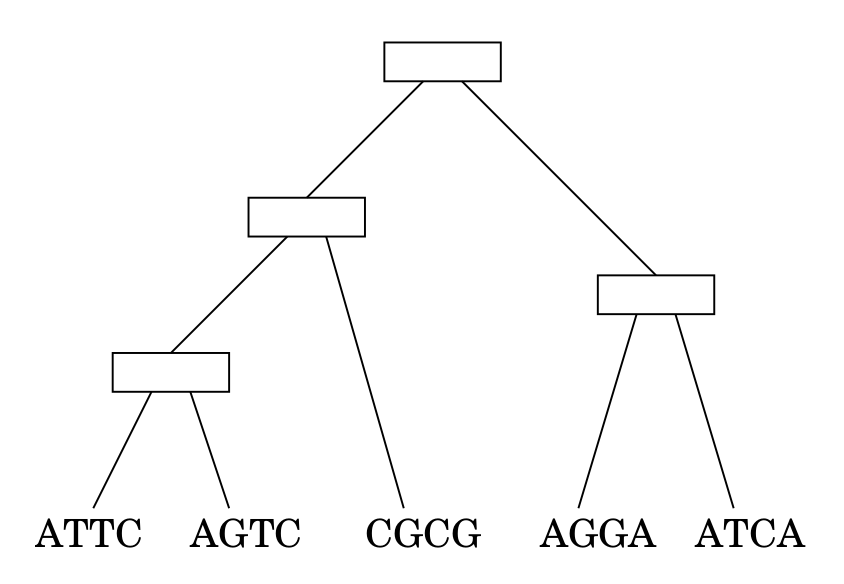
\includegraphics[width=.9\linewidth]{6_30/tree.png}}

\begin{enumerate}
\item Ache uma reconstrução para o exemplo seguindo o método da
máxima parcimônia.
\item Dê um algoritmo eficiente para essa tarefa.
\end{enumerate}

\section{Solução}
\label{sec-2}

Como o valor só depende TODO. Vamos calcular a resposta para cada
letra independentemente e depois concatenar as respostas para obter a
árvore final.

Nós vamos usar um algoritmo de programação dinâmica para encontrar o
valor das folhas intermediárias em uma árvore $P$ em que cada
folha tem valor A, G, T ou C

TODO: estrutura de dados para representar a árvore.
\begin{minted}[]{python}
# Colocar aqui uma estrutura de dados para a arvore
\end{minted}

TODO: achar um nome melhor para ans

Vamos computar $ans[v][\ell]$ como a melhor maneira de preencher os nós
da sub-árvore enraizada em $v$, dado que o pai de $v$ tem valor $\ell$.

TODO: justificar a inicializacao
\begin{minted}[]{python}
valor = {}
ans = {}
\end{minted}

Vamos computar $ans$ de baixo para cima. Então, o caso base para esse algoritmo
é a resposta para as folhas, isso é, $ans[\mathrm{folha}][\ell]$.

Uma sub-árvore que contém apenas uma folha e seu pai vai ter
$\mathrm{nota} = 0$ se a folha e o pai tiverem ambos o mesmo valor (A,
G, T ou C) ou $\mathrm{nota} = 1$, se os dois tiverem valores diferentes:

\[ans[\mathrm{folha}][\ell] = \begin{cases}0 \text{ se } \mathrm{valor}[\mathrm{folha}] = \ell \\
                                                     1 \text{ caso contrário}\end{cases}\]

Podemos então preencher as folhas:
\begin{minted}[]{python}
#TODO: preencher as folhas
\end{minted}

Tendo o caso base, podemos computar $ans[v][\ell]$ assumindo que $ans[w][\ell]$ já foi computado para
todo $w$ filho de $v$ e $\ell \in \{A, G, T, C\}$.

TODO: explicar em algum lugar que a raiz é especial

A nota da sub-árvore quando o valor de $v$ é igual a $m$ é:

\[[\ell \neq m] + \sum_{w \text{ filho de }v} ans[w][m]\]

Onde \[[\ell \neq m] =  \begin{cases} 0 \text{ se } m = \ell \\
                                     1 \text{ caso contrário}\end{cases}\]

Queremos escolher um valor $m \in \{A, G, T, C\}$ para $v$
que minimize a nota final da sub-árvore. Então:

\[ans[v][\ell] = \min_{m \in \{A, G, T, C\}}  \left([\ell \neq m] + \sum_{w \text{ filho de }v} ans[w][m]\right)\]

\begin{minted}[]{python}
# TODO: preencher os outros vértices (exceto a raiz)
\end{minted}

Após computarmos $ans[v][\ell]$ para todos os vértices exceto a raiz
podemos encontrar a nota da árvore como o mínimo entre os possíveis
valores para a raiz:

\[ \min_{\ell \in \{A, G, T, C\}} \sum_{v \text{ filho da raiz}} ans[v][\ell]\]


\section{Dados reais}
\label{sec-3}

\subsection{Formato Newick}
\label{sec-3-1}

Um formato muito usado para árvores em bioinformática é o formato
Newick. Assim como LISP, ele usa o fato de que parenteses podem ser
usados para especificar uma árvore.

TODO: especificar o formato, referência do formato

\subsubsection{Parseando o formato Newick}
\label{sec-3-1-1}

\subsection{Rosalind}
\label{sec-3-2}

Obtemos os dados do Rosalind, TODO: explicar o Rosalind.

Rosalind MULT, GLOB, EDTA, PERM, EDIT, LCSQ,
CSTR, CTBL, NWCK, SSET, MRNA, KMP, PROB
SSEQ, SPLC, LCSM

\subsection{Rodando o algoritmo com dados reais}
\label{sec-3-3}

\section{Extensões}
\label{sec-4}

Ao fazer esse exercício, notamos que a árvore já é uma entrada do problema.
Como é possível obter a árvore de menor valor a partir das espécies

Esse problema é NP-completo [TODO: colocar referência] e o melhor
algoritmo conhecido é [TODO]
% Emacs 24.4.1 (Org mode 8.2.10)
\end{document}
